\documentclass[border=6pt]{standalone}
\usepackage[utf8]{inputenc}\usepackage[T1]{fontenc}\usepackage{lmodern}
\usepackage{tikz}\usetikzlibrary{shapes.geometric,calc}
\definecolor{facervo}{HTML}{DCE9F5}\definecolor{sacervo}{HTML}{3D6E9E}
\definecolor{fuser}{HTML}{E4DEF2}\definecolor{suser}{HTML}{6A5A94}
\definecolor{faval}{HTML}{FAE3CE}\definecolor{saval}{HTML}{B0703A}
\definecolor{fponte}{HTML}{E2EFD9}\definecolor{sponte}{HTML}{5A8542}
\definecolor{fneut}{HTML}{FFFFFF}\definecolor{sneut}{HTML}{5A6570}
\definecolor{fattr}{HTML}{FFFFFF}\definecolor{sattr}{HTML}{7A848C}
\begin{document}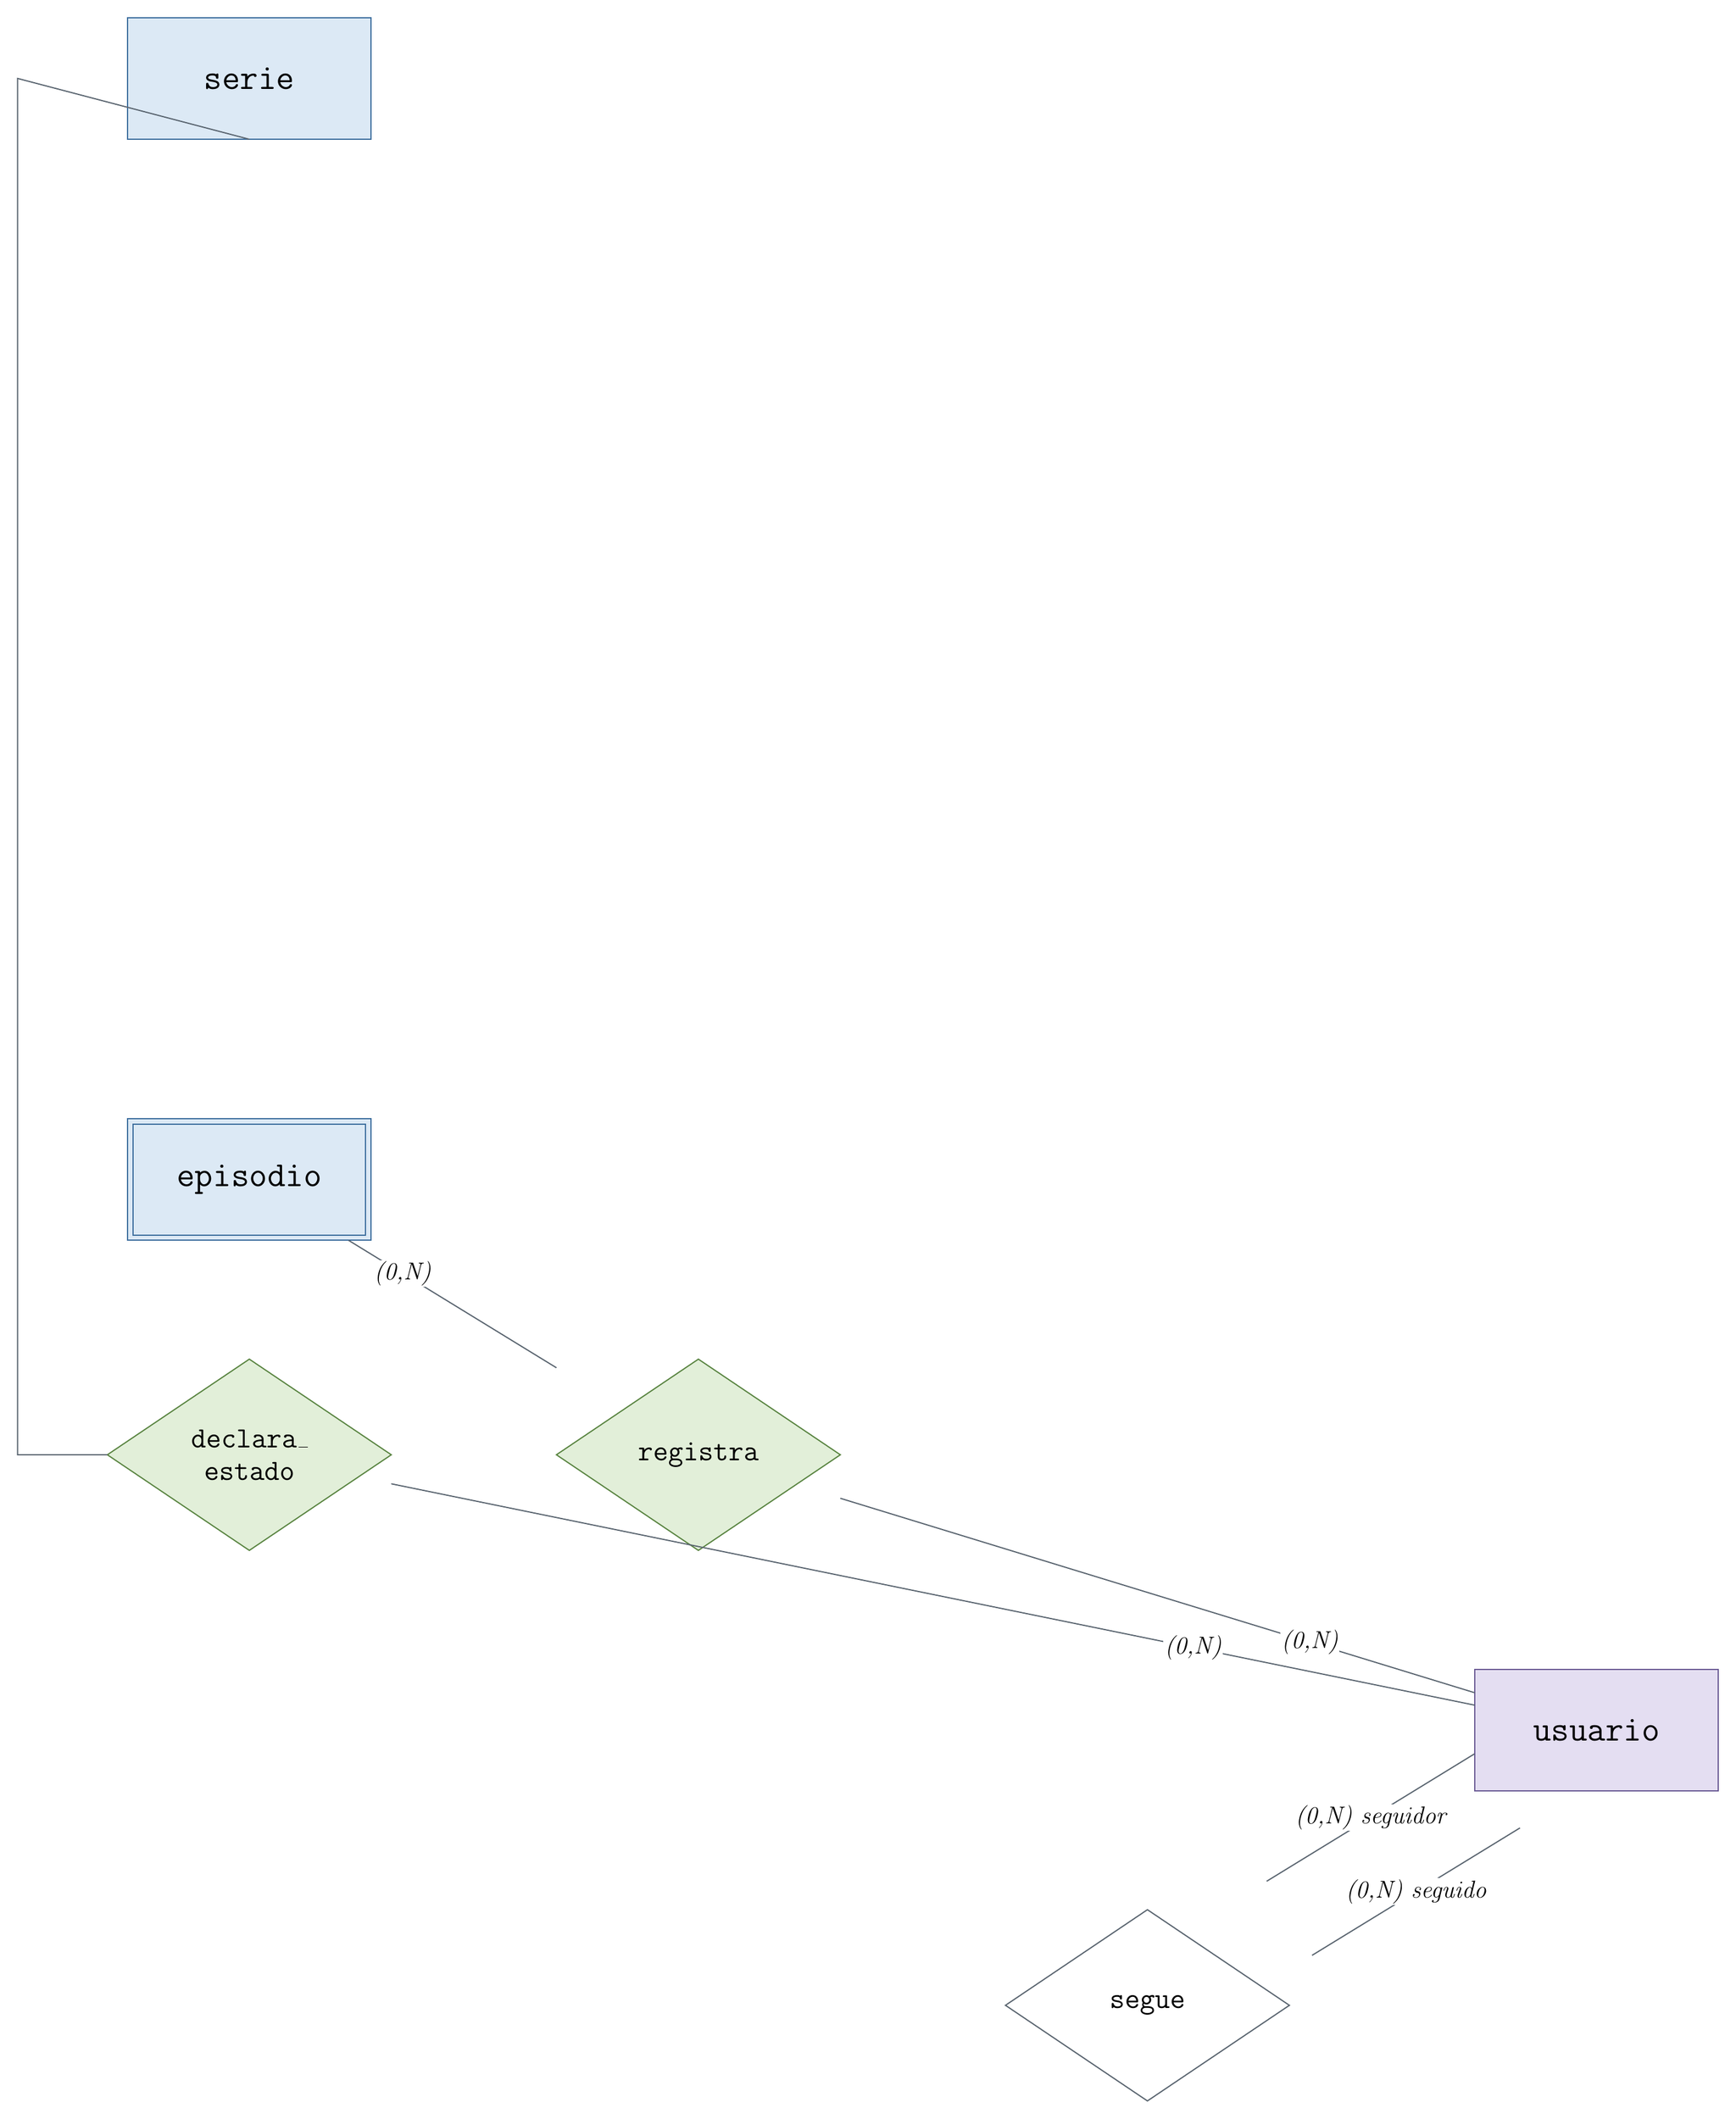
\begin{tikzpicture}[line width=0.7pt]
\draw[fill=facervo,draw=sacervo] ($ (4.800,-37.500) + (-2.520,-1.260) $) rectangle ($ (4.800,-37.500) + (2.520,1.260) $);
\draw[draw=sacervo] ($ (4.800,-37.500) + (-2.410,-1.150) $) rectangle ($ (4.800,-37.500) + (2.410,1.150) $);
\node at (4.800,-37.500) {\fontsize{19.63}{23.17}\selectfont\ttfamily episodio};
\draw[fill=facervo,draw=sacervo] ($ (4.800,-14.700) + (-2.520,-1.260) $) rectangle ($ (4.800,-14.700) + (2.520,1.260) $);
\node at (4.800,-14.700) {\fontsize{19.63}{23.17}\selectfont\ttfamily serie};
\draw[fill=fneut,draw=sneut] ($ (23.400,-54.600) + (0,1.980) $) -- ($ (23.400,-54.600) + (2.940,0) $) -- ($ (23.400,-54.600) + (0,-1.980) $) -- ($ (23.400,-54.600) + (-2.940,0) $) -- cycle;
\node at (23.400,-54.600) {\fontsize{16.22}{19.14}\selectfont\ttfamily segue};
\draw[fill=fponte,draw=sponte] ($ (4.800,-43.200) + (0,1.980) $) -- ($ (4.800,-43.200) + (2.940,0) $) -- ($ (4.800,-43.200) + (0,-1.980) $) -- ($ (4.800,-43.200) + (-2.940,0) $) -- cycle;
\node at (4.800,-42.864) {\fontsize{16.22}{19.14}\selectfont\ttfamily declara\_};
\node at (4.800,-43.536) {\fontsize{16.22}{19.14}\selectfont\ttfamily estado};
\draw[fill=fponte,draw=sponte] ($ (14.100,-43.200) + (0,1.980) $) -- ($ (14.100,-43.200) + (2.940,0) $) -- ($ (14.100,-43.200) + (0,-1.980) $) -- ($ (14.100,-43.200) + (-2.940,0) $) -- cycle;
\node at (14.100,-43.200) {\fontsize{16.22}{19.14}\selectfont\ttfamily registra};
\draw[fill=fuser,draw=suser] ($ (32.700,-48.900) + (-2.520,-1.260) $) rectangle ($ (32.700,-48.900) + (2.520,1.260) $);
\node at (32.700,-48.900) {\fontsize{19.63}{23.17}\selectfont\ttfamily usuario};
\draw[draw=sneut] (6.856,-38.760) -- (11.160,-41.398);
\draw[draw=sneut] (17.040,-44.101) -- (30.180,-48.128);
\draw[draw=sneut] (4.800,-15.960) -- (0.000,-14.700) -- (0.000,-43.200) -- (1.860,-43.200);
\draw[draw=sneut] (7.740,-43.801) -- (30.180,-48.385);
\draw[draw=sneut] (30.174,-49.393) -- (25.870,-52.031);
\draw[draw=sneut] (26.810,-53.565) -- (31.115,-50.927);
\node[fill=white,inner sep=0.7pt] at (7.975,-39.446) {\fontsize{13.66}{16.12}\selectfont\itshape (0,N)};
\node[fill=white,inner sep=0.7pt] at (26.764,-47.081) {\fontsize{13.66}{16.12}\selectfont\itshape (0,N)};
\node[fill=white,inner sep=0.7pt] at (24.346,-47.193) {\fontsize{13.66}{16.12}\selectfont\itshape (0,N)};
\node[fill=white,inner sep=0.7pt] at (28.022,-50.712) {\fontsize{13.66}{16.12}\selectfont\itshape (0,N) seguidor};
\node[fill=white,inner sep=0.7pt] at (28.962,-52.246) {\fontsize{13.66}{16.12}\selectfont\itshape (0,N) seguido};
\end{tikzpicture}\end{document}